\chapter{Common Distributions and Their Properties}\label{ch:distributions}
%!TEX root = main.tex

This chapter is a reference for the standard distributions encountered in statistical inference.  Although you are encouraged to read this chapter through, it can also be read out-of-order to look at a specific distribution.

\section{Discrete and Continuous}

Some distributions apply to a discrete (i.e. countable) number of possibilities while others apply to continuous values.  In the case of discrete variables, the probability is given by the actual value of the distribution, so it makes sense to speak of the probability of an individual label, $P({\rm coin 1})$.  In the case of continuous variables, the probability is given by the area under the distribution, so it makes sense only to speak of the probability if a range of labels, $P(0.2 < \theta < 0.3)$. 

\section{Uniform}

\subsection{Discrete}

\highlight{Discrete uniform distribution}{The discrete uniform distribution is defined to be a {\em constant} value for all possibilities.  Mathematically this is written \[p(x_{i})=\frac{1}{N}\] where $N$ is the total number of possibilities, labeled $x_{1}$ to $x_{N}$.  The picture of the distribution is shown in Figure~\ref{fig:uniform_discrete}}{The discrete uniform distribution is defined to be a {\em constant} value for all possibilities.  Mathematically this is written \[p(x_{i})=\frac{1}{N}\] where $N$ is the total number of possibilities, labeled $x_{1}$ to $x_{N}$.}

\begin{figure}
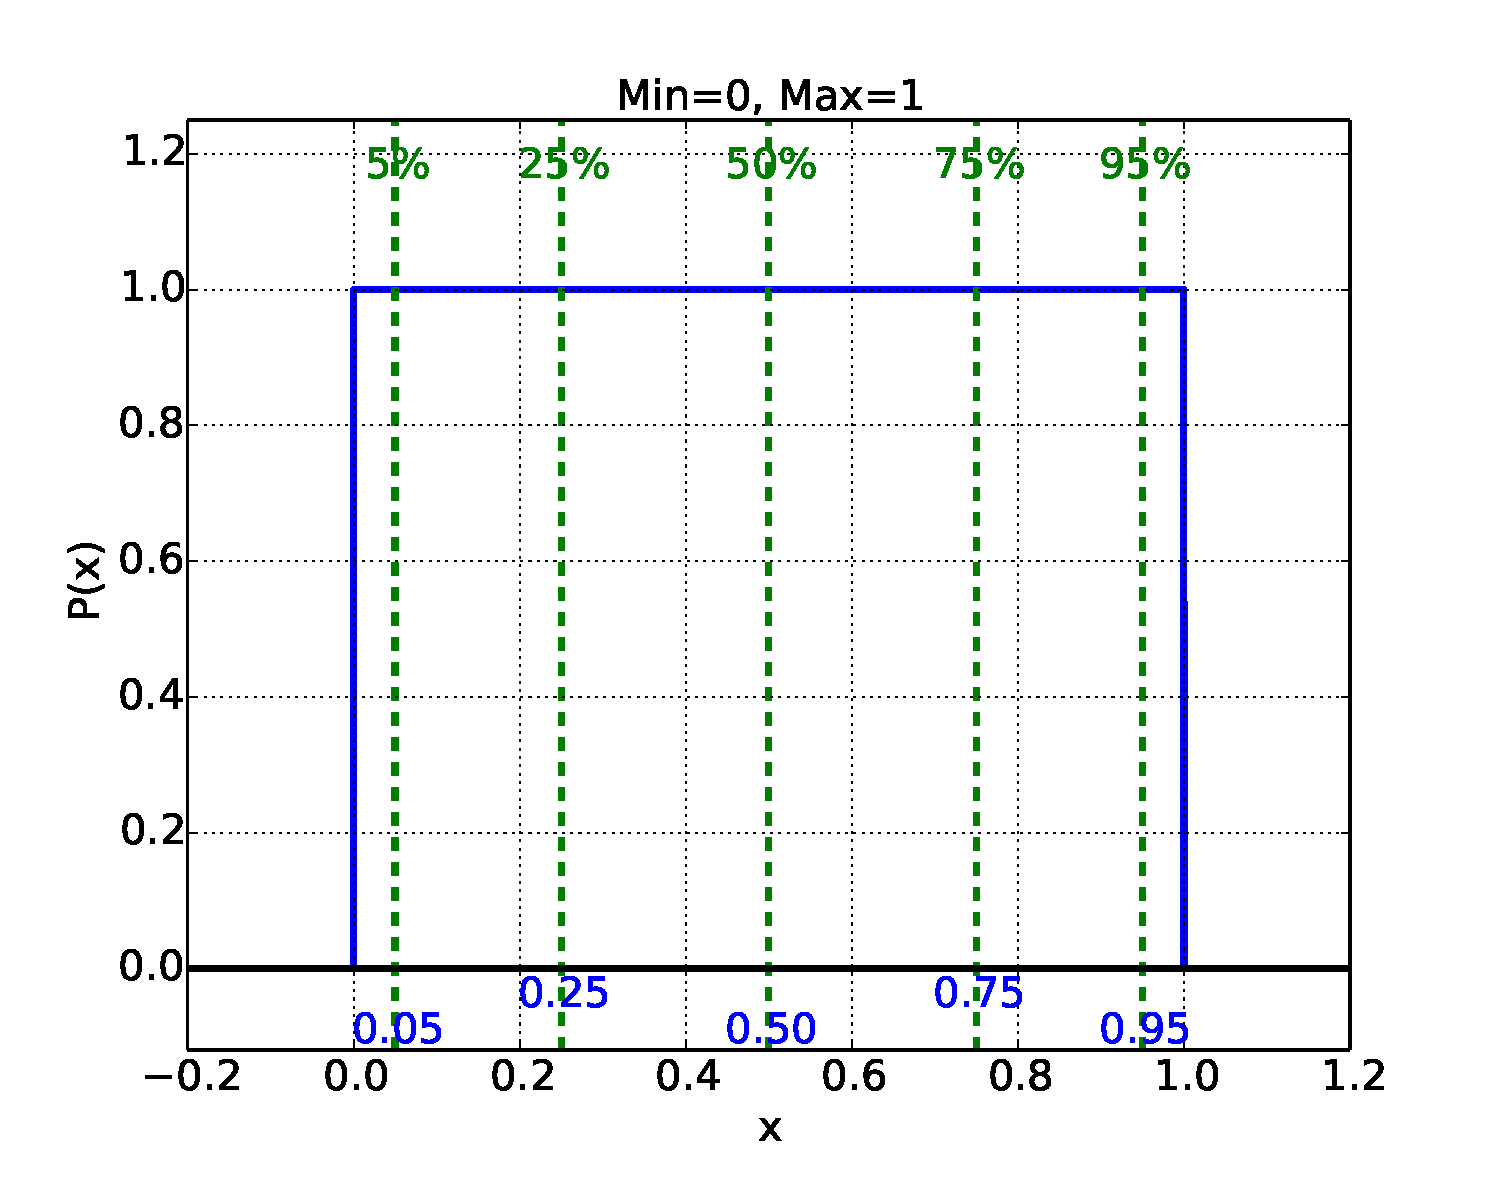
\includegraphics[width=4.8in]{distributions_1}
\label{fig:uniform_discrete}
\caption{Discrete uniform distribution for values 1 to 6.  The value for each is $p(x_{i})=1/6$.}
\end{figure}

\subsection{Continuous}


\highlight{Continuous uniform distribution}{The continuous uniform distribution is defined to be a {\em constant} between a minimum and maximum value, and zero everywhere else.  Mathematically this is written \[p(x)=\frac{1}{\rm max-min} \mbox{ for }{\rm min}<x<{\rm max}\].  The picture of the distribution is shown in Figure~\ref{fig:uniform_continuous}.}{
The continuous uniform distribution is defined to be a {\em constant} between a minimum and maximum value, and zero everywhere else.  Mathematically this is written \[p(x)=\frac{1}{\rm max-min} \mbox{ for }{\rm min}<x<{\rm max}\].
}
\begin{figure}
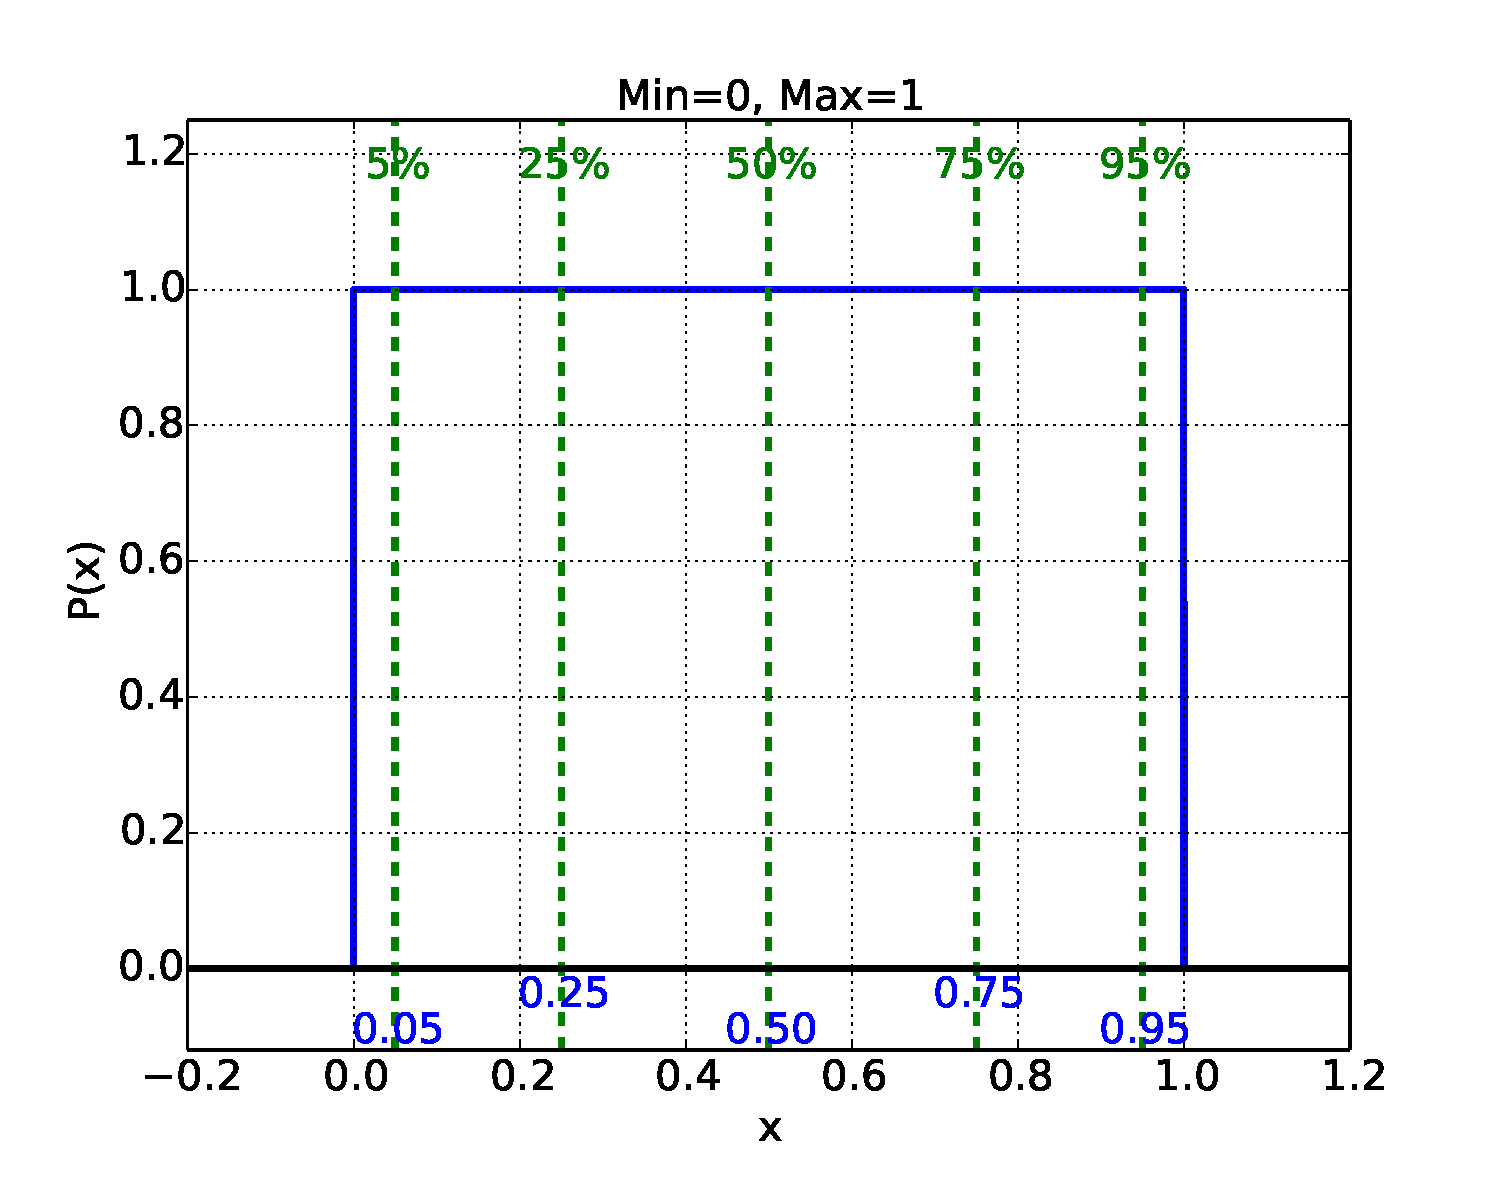
\includegraphics[width=4.8in]{distributions_1}
\label{fig:uniform_continuous}
\caption{Continuous uniform distribution between values 0 and 1}
\end{figure}



\example{
You call a plumber, and they say that they can come anytime in the next 4 hours.  The probability of them arriving at any particular time can be represented with a uniform distribution.  What is the probability that they arrive in the first 20 minutes of the second hour?
\label{ex:plumber}}


\begin{figure}
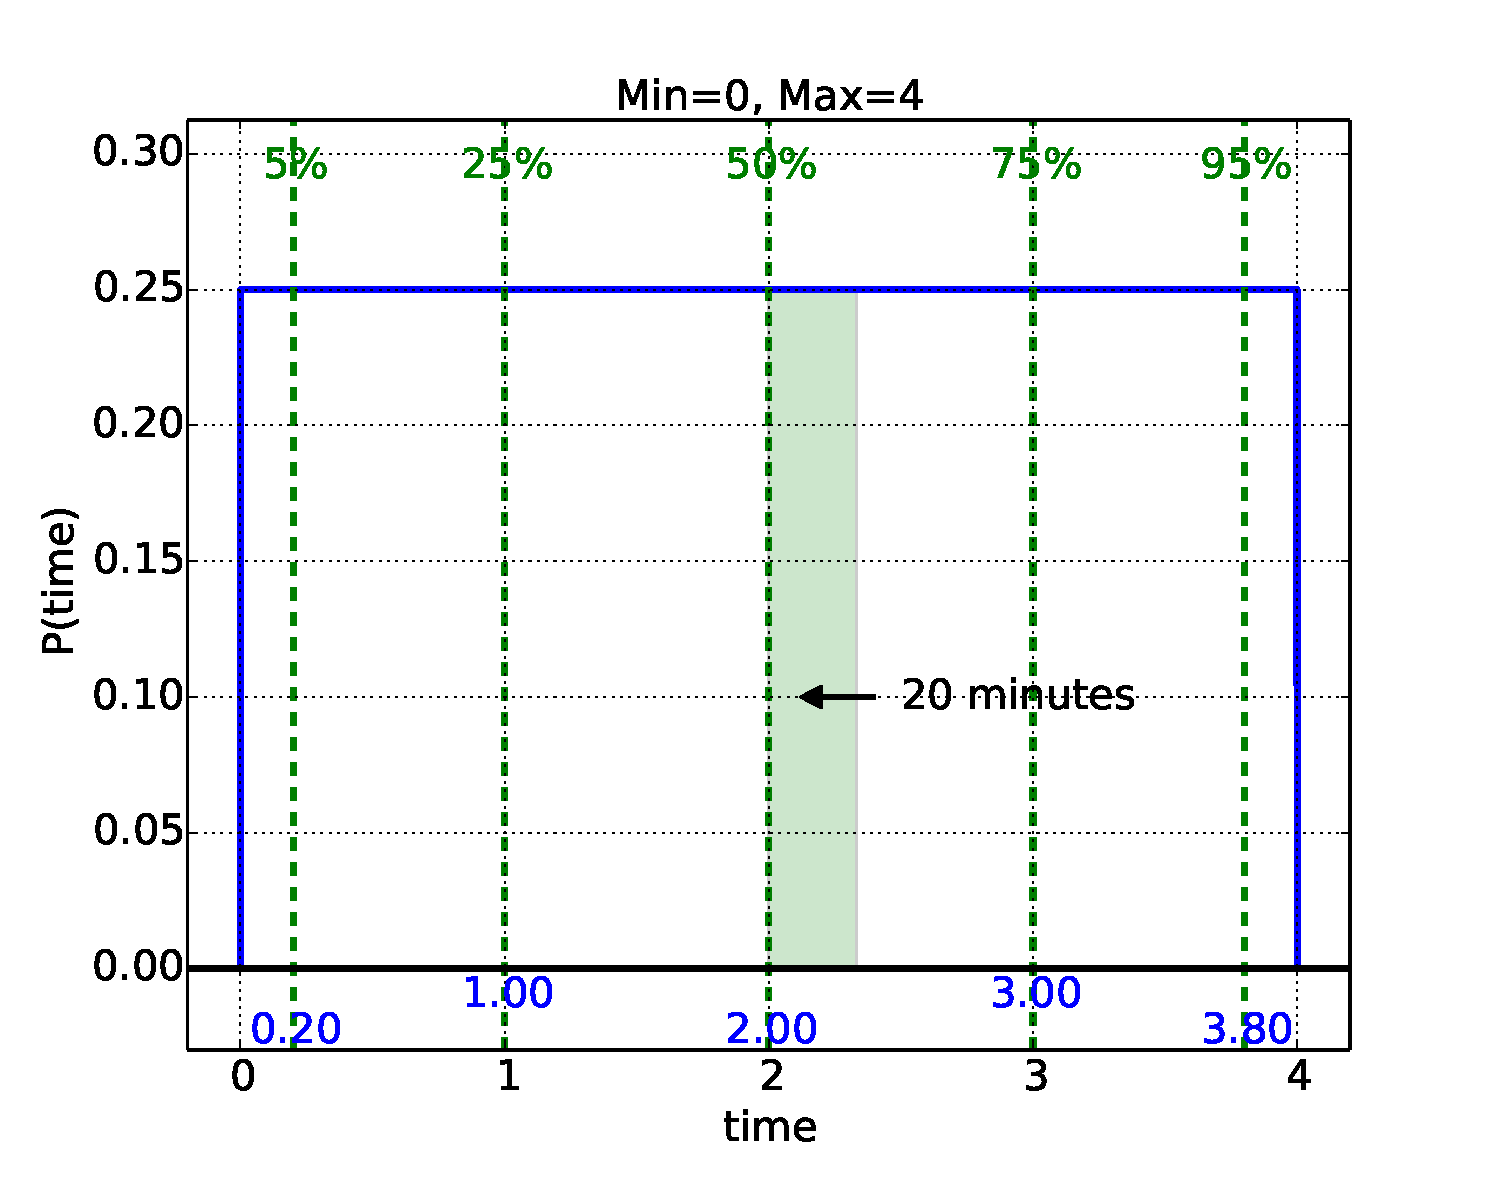
\includegraphics[width=4.8in]{distributions_plumber}
\label{fig:uniform_plumber}
\caption{Continuous uniform distribution for the plumber example (Example~\ref{ex:plumber}).}
\end{figure}


In order to ask questions about total probability from a {\em continuous} distribution you take the {\em area under the curve} between the relevant values.\marginnote{The reason for the particular constant value for the uniform distribution, $1/(\rm max-min)$, is simply that the area of the entire rectangle must be 1, which means that there is a 100\% chance of the values falling between the minimum and maximum values.}  In this case it'd be the area under the curve from the time $t=2 {\rm hr}$ and $t=2 {\rm hr} + 20 {\rm minutes} = 2.333 {\rm hr}$, as shown in Figure~\ref{fig:uniform_plumber}.  The area under the curve is just the area of the shaded region between times $t=2{\rm hr}$ and $t=2.333 {\rm hr}$, or just the area of a rectangle - $A={\rm base} \times {\rm height}$.  The {\em base} of the rectangle is the length of time, or \beqn
\mbox{{\em base}}=0.333 {\rm hr}
\eeqn
The {\rm height} of the rectangle is given by the constant value of the uniform distribution, or \beqn
\mbox{{\em height}} = \frac{1}{{\rm max}-{\rm min}} = \frac{1}{4 {\rm hr} - 0 {\rm hr}} = 0.25 \frac{1}{\rm hr}
\eeqn
So the total probability of the plumber coming in the first 20 minutes of the second hour is
\beqn
P(2<t<2.25) = \left(0.333 {\rm hr}\right) \times \left(0.25 \frac{1}{\rm hr}\right) = 0.0833
\eeqn

\section{Binomial}

\highlight{Binomial distribution}{The discrete binomial distribution  is defined to be the probability of achieving $h$ successes in a given $N$ events where each event has a given $\theta$ probability of success.

\beqn
P(h|N,\theta) = \nchoosek{h}{N} \theta^{h} (1-\theta)^{N-h}
\eeqn
}{The discrete binomial distribution  is defined to be the probability of achieving $h$ successes in a given $N$ events where each event has a given $\theta$ probability of success.

\beqn
P(h|N,\theta) = \nchoosek{h}{N} \theta^{h} (1-\theta)^{N-h}
\eeqn
}

\begin{figure}
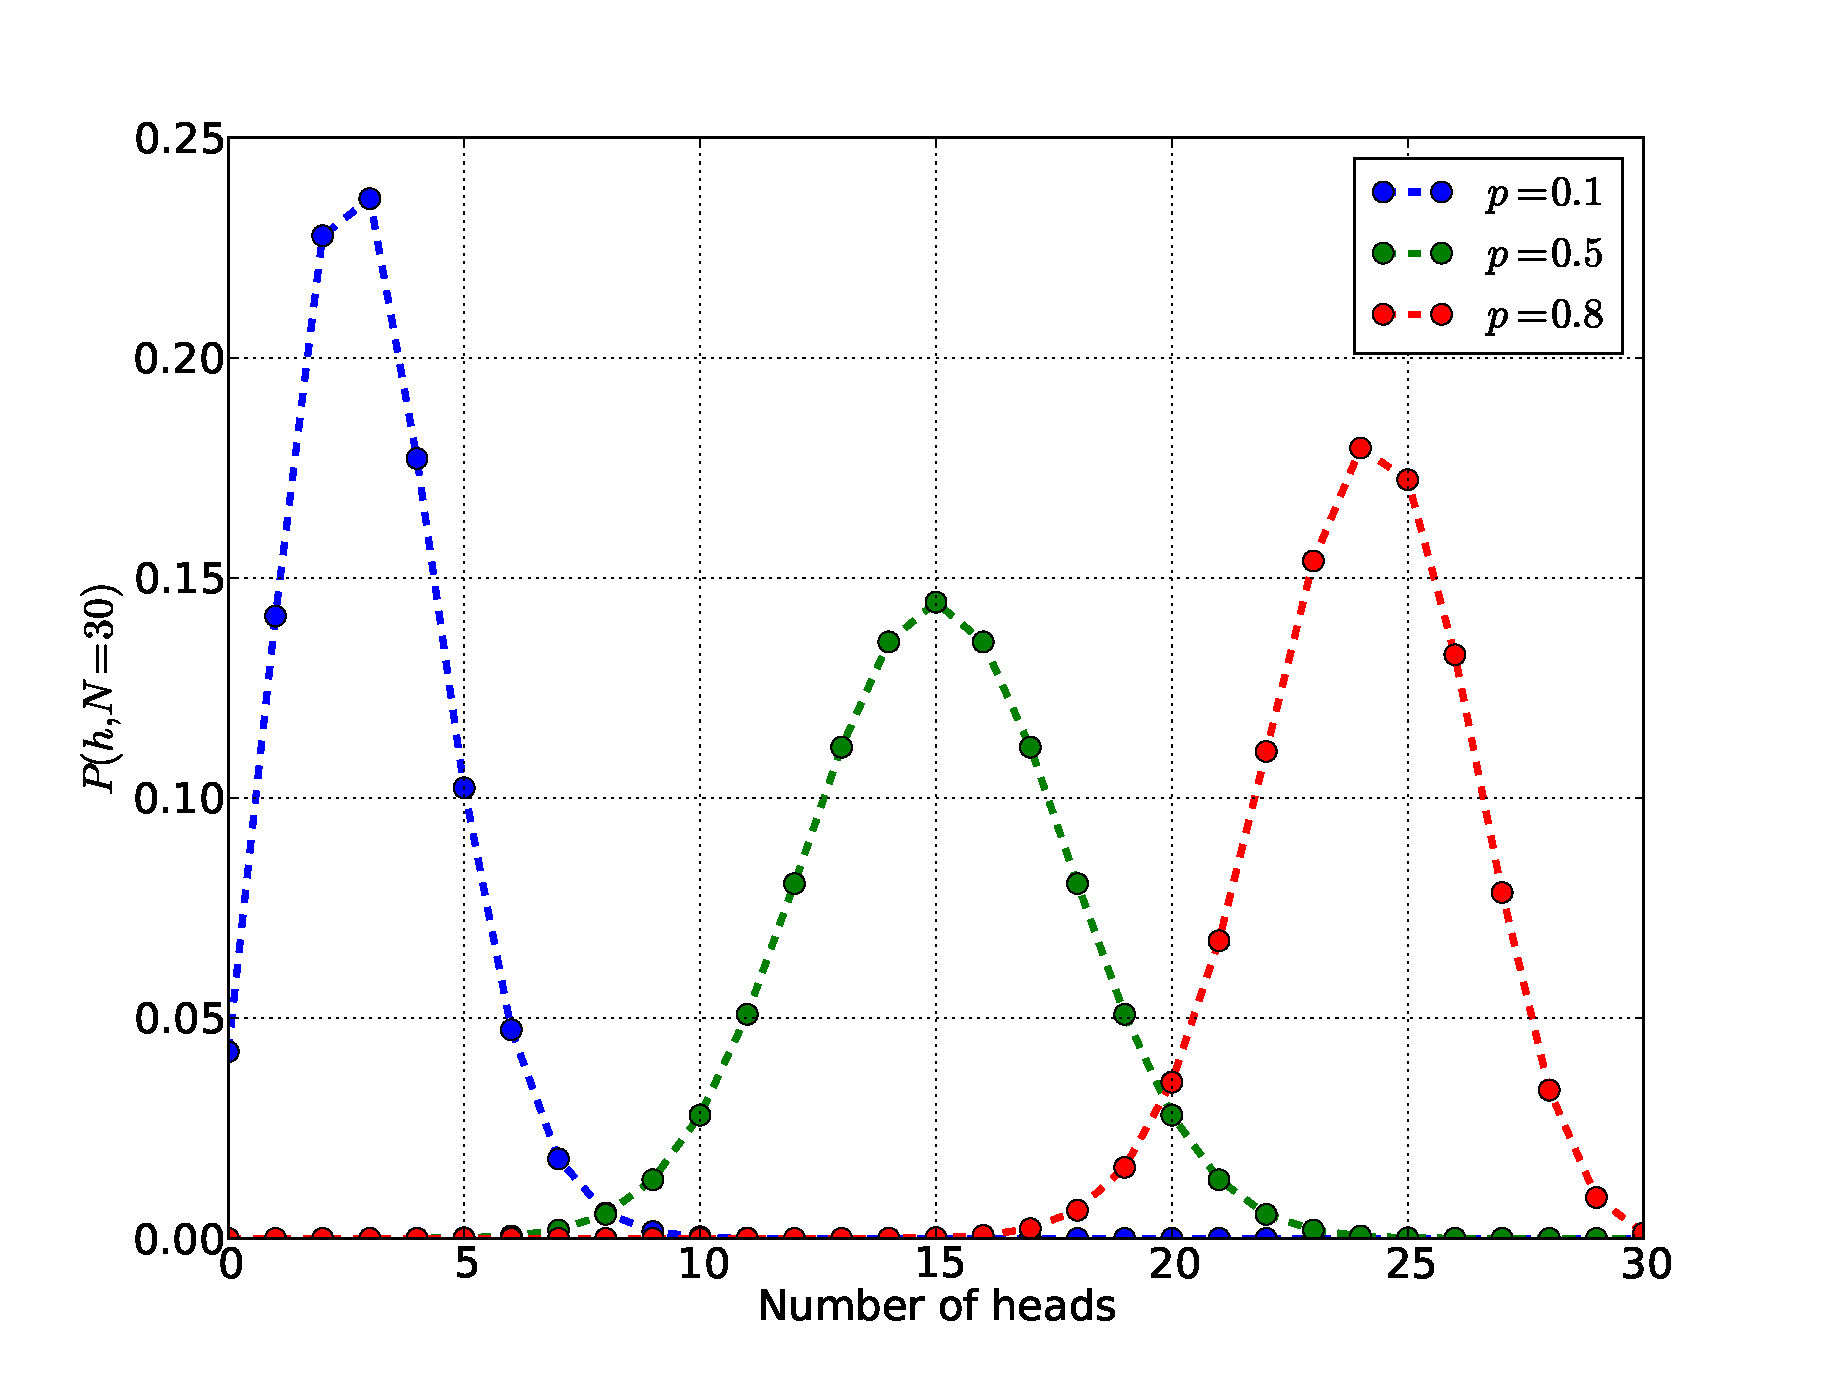
\includegraphics{coinflips5}
\caption{Probability of getting $h$ heads in 30 flips given a possible unfair coin. One coin has $p=0.1$, where the maximum is for 3 heads (or 1/10 of the 30 flips), but 2 heads is nearly as likely.  Another has $p=0.5$, and is the fair coin considered earlier with a maximum at 15 heads (or 1/2 of the 30 flips).  Finally, another coin shown as $p=0.8$ where 24 heads (or 8/10 of the 30 flips) is maximum. }
\label{fig:binomial_dist}
\end{figure}

Although it may look like a Beta, the binomial distribution is used to find the best estimate for the number of successes, $h$, given the number of events, $N$, and the probability of the success of a single event, $\theta$. 


\section{Beta}

\highlight{Beta distribution}{The continuous Beta distribution is the posterior probability distribution for the parameter $\theta$, where one has observed $h$ successes in a given $N$ events, and each event is assumed to have a $\theta$ probability of success.

\beqn
P(\theta|h,N) = (N+1)\cdot \nchoosek{N}{h} \theta^{h} (1-\theta)^{N-h}
\eeqn
}{The continuous Beta distribution is the posterior probability distribution for the parameter $\theta$, where one has observed $h$ successes in a given $N$ events, and each event is assumed to have a $\theta$ probability of success.

\beqn
P(\theta|h,N) = (N+1)\cdot \nchoosek{N}{h} \theta^{h} (1-\theta)^{N-h}
\eeqn
}

Although it may look like a binomial, the Beta distribution is used to find the best estimate for the parameter $\theta$ where the number of successes and events, $h$ and $N$ are given.


\begin{figure}
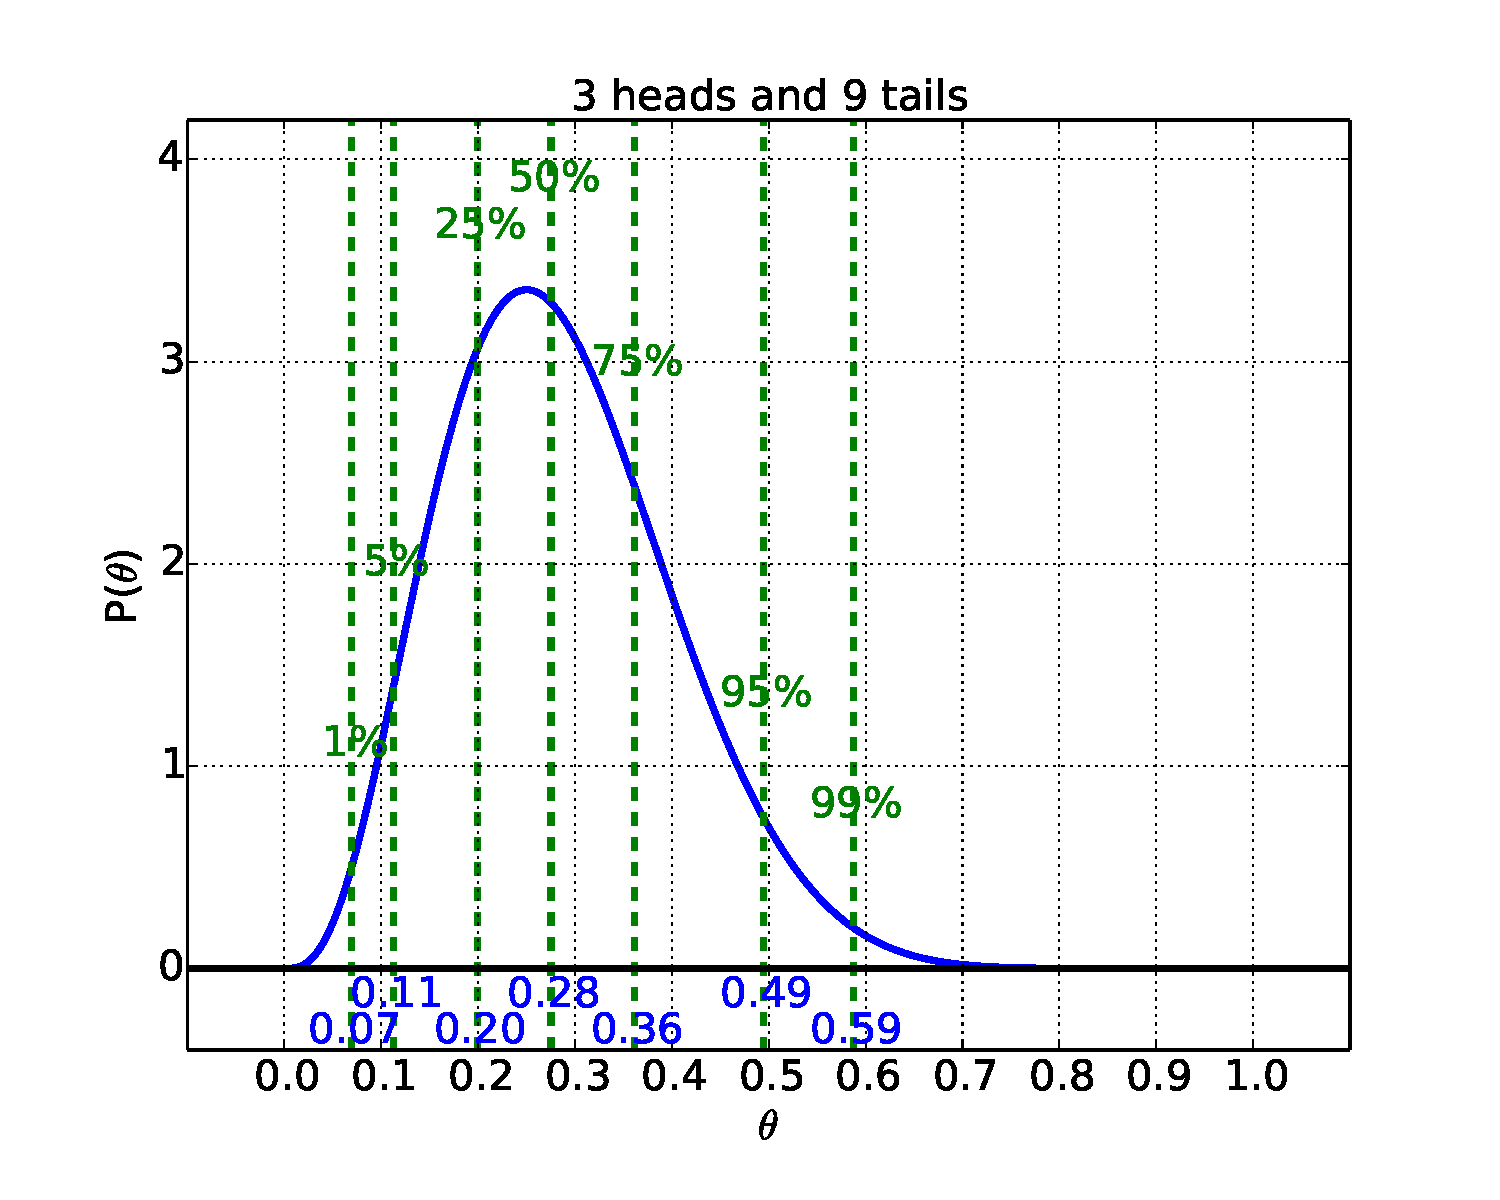
\includegraphics{beta_dist4}
\caption{Posterior probability distribution for the $\theta$ values of the bent coin - the probability that the coin will land heads.  The distribution is shown for data 3 heads and 9 tails.  The various quartiles are shown in the plot.}
\label{fig:beta_dist}
\end{figure}


\section{Normal (Gaussian)}

\begin{figure}
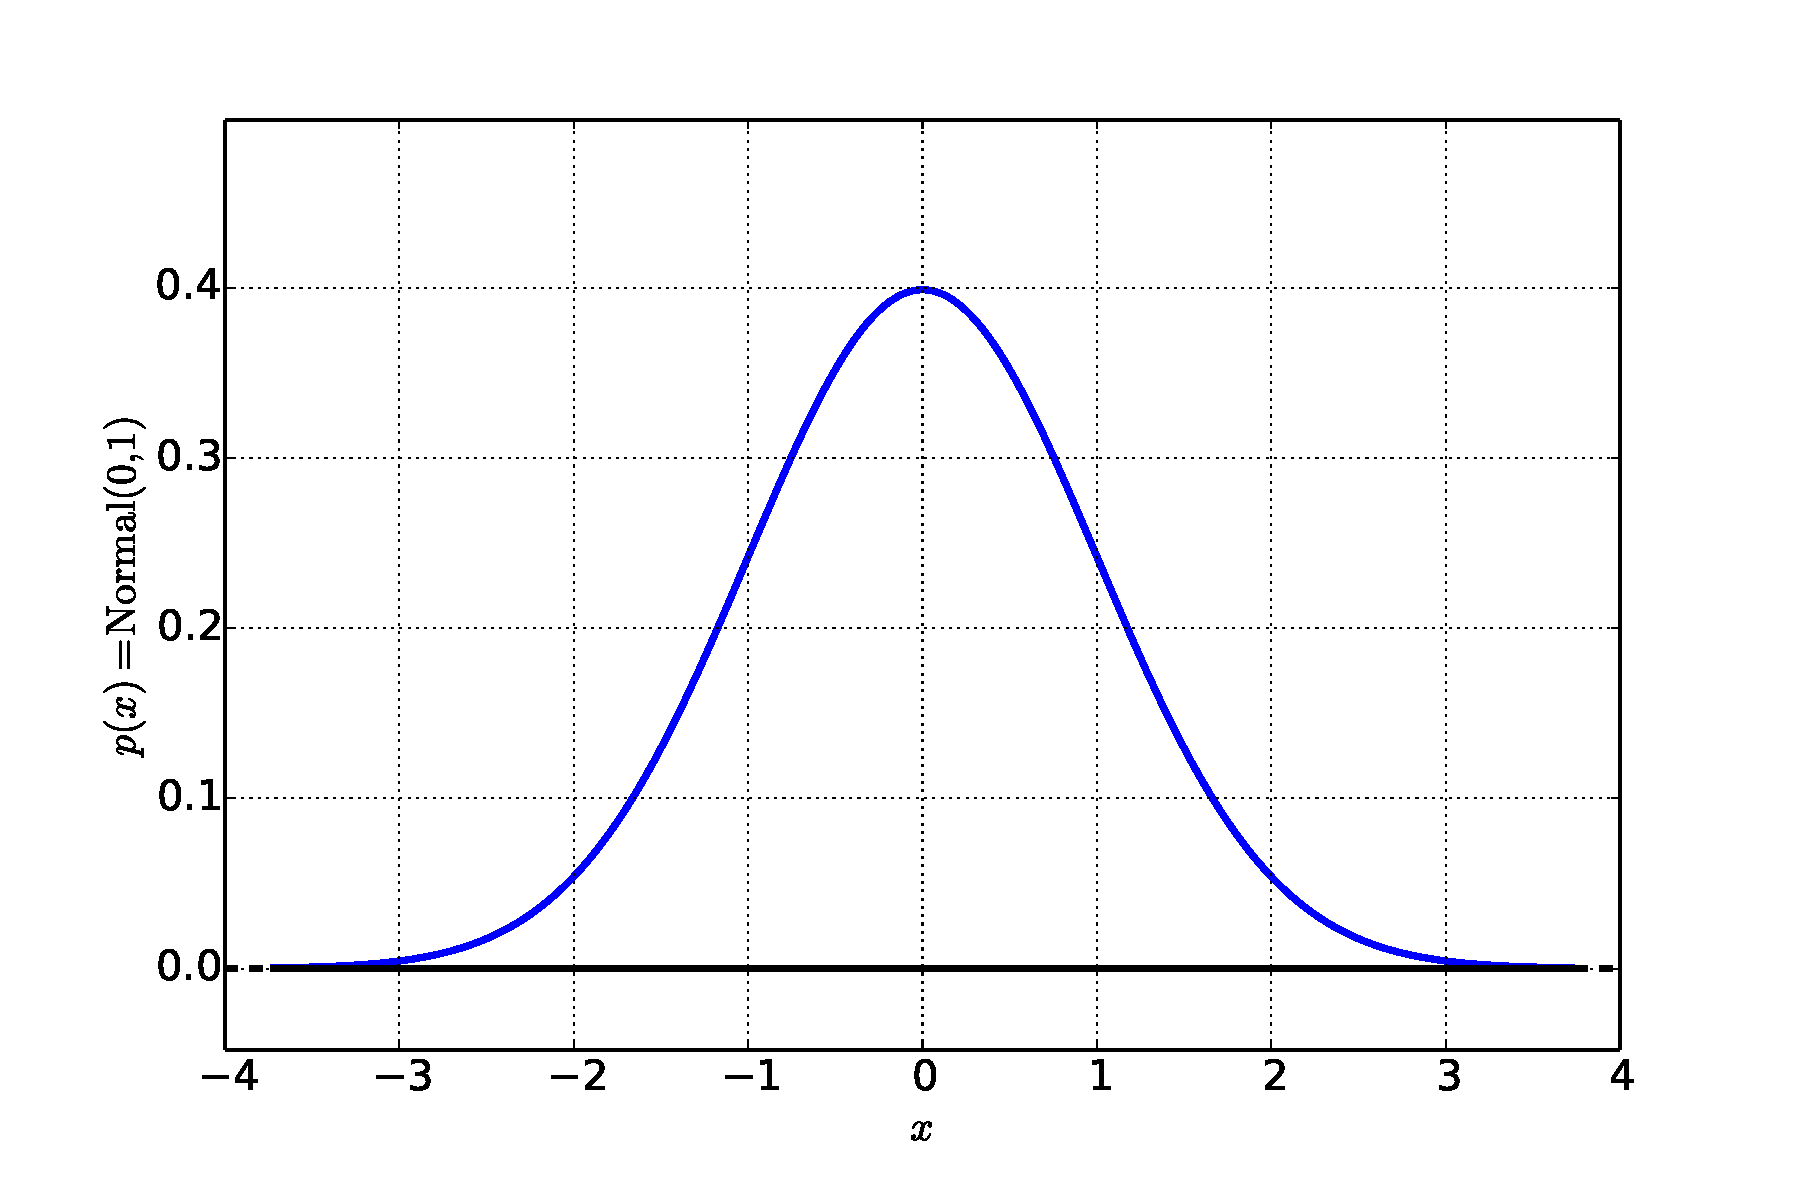
\includegraphics{gaussian1}
\caption{The normal distribution.}
\label{fig:bell_appendix}
\end{figure}

\highlight{Normal distribution}{The Normal distribution is the most common distribution found in all of statistical inference.  It is the best prior distribution to use, when all you know is that your data has a constant true value and some constant variation around that true value.  It is the posterior probability distribution for the unknown true value given $N$ samples and the known deviation, $\sigma$.  It is also the approximate form for nearly every distribution when you have many samples.  The mathematical form for the normal, or Gaussian, is

\beqn
{\rm Normal}(\mu,\sigma) = \frac{1}{\sqrt{2\pi\sigma^{2}}} e^{-(x-\mu)^{2}/2\sigma^{2}}
\eeqn

}{The Normal distribution is the most common distribution found in all of statistical inference.  It is the best prior distribution to use, when all you know is that your data has a constant true value and some constant variation around that true value.  It is the posterior probability distribution for the unknown true value given $N$ samples and the known deviation, $\sigma$.  It is also the approximate form for nearly every distribution when you have many samples.  The mathematical form for the normal, or Gaussian, is

\beqn
{\rm Normal}(\mu,\sigma) = \frac{1}{\sqrt{2\pi\sigma^{2}}} e^{-(x-\mu)^{2}/2\sigma^{2}}
\eeqn
}


Three useful properties of $\sigma$ for the normal distribution are the following:
\be
\i the normal distribution value at the maximum (i.e. at $x=\mu$) is around 2.7 times larger than the value one-$\sigma$ away from the maximum (at $x=\mu-\sigma$ and $x=\mu+\sigma$)
\i the total probability between these two points is 65\%.  
\i 95\% of the distribution lies between $\mu-2\sigma$ and $\mu+2\sigma$ (see Figure~\ref{fig:gaussian_sigma})
\ee

\comment{

\section{Student's {\em t}}

The Student's {\em t} distribution is the posterior distribution for the true value, $\mu$, of a quantity given $N$ samples and unknown deviation, $\sigma$. 


\begin{figure}
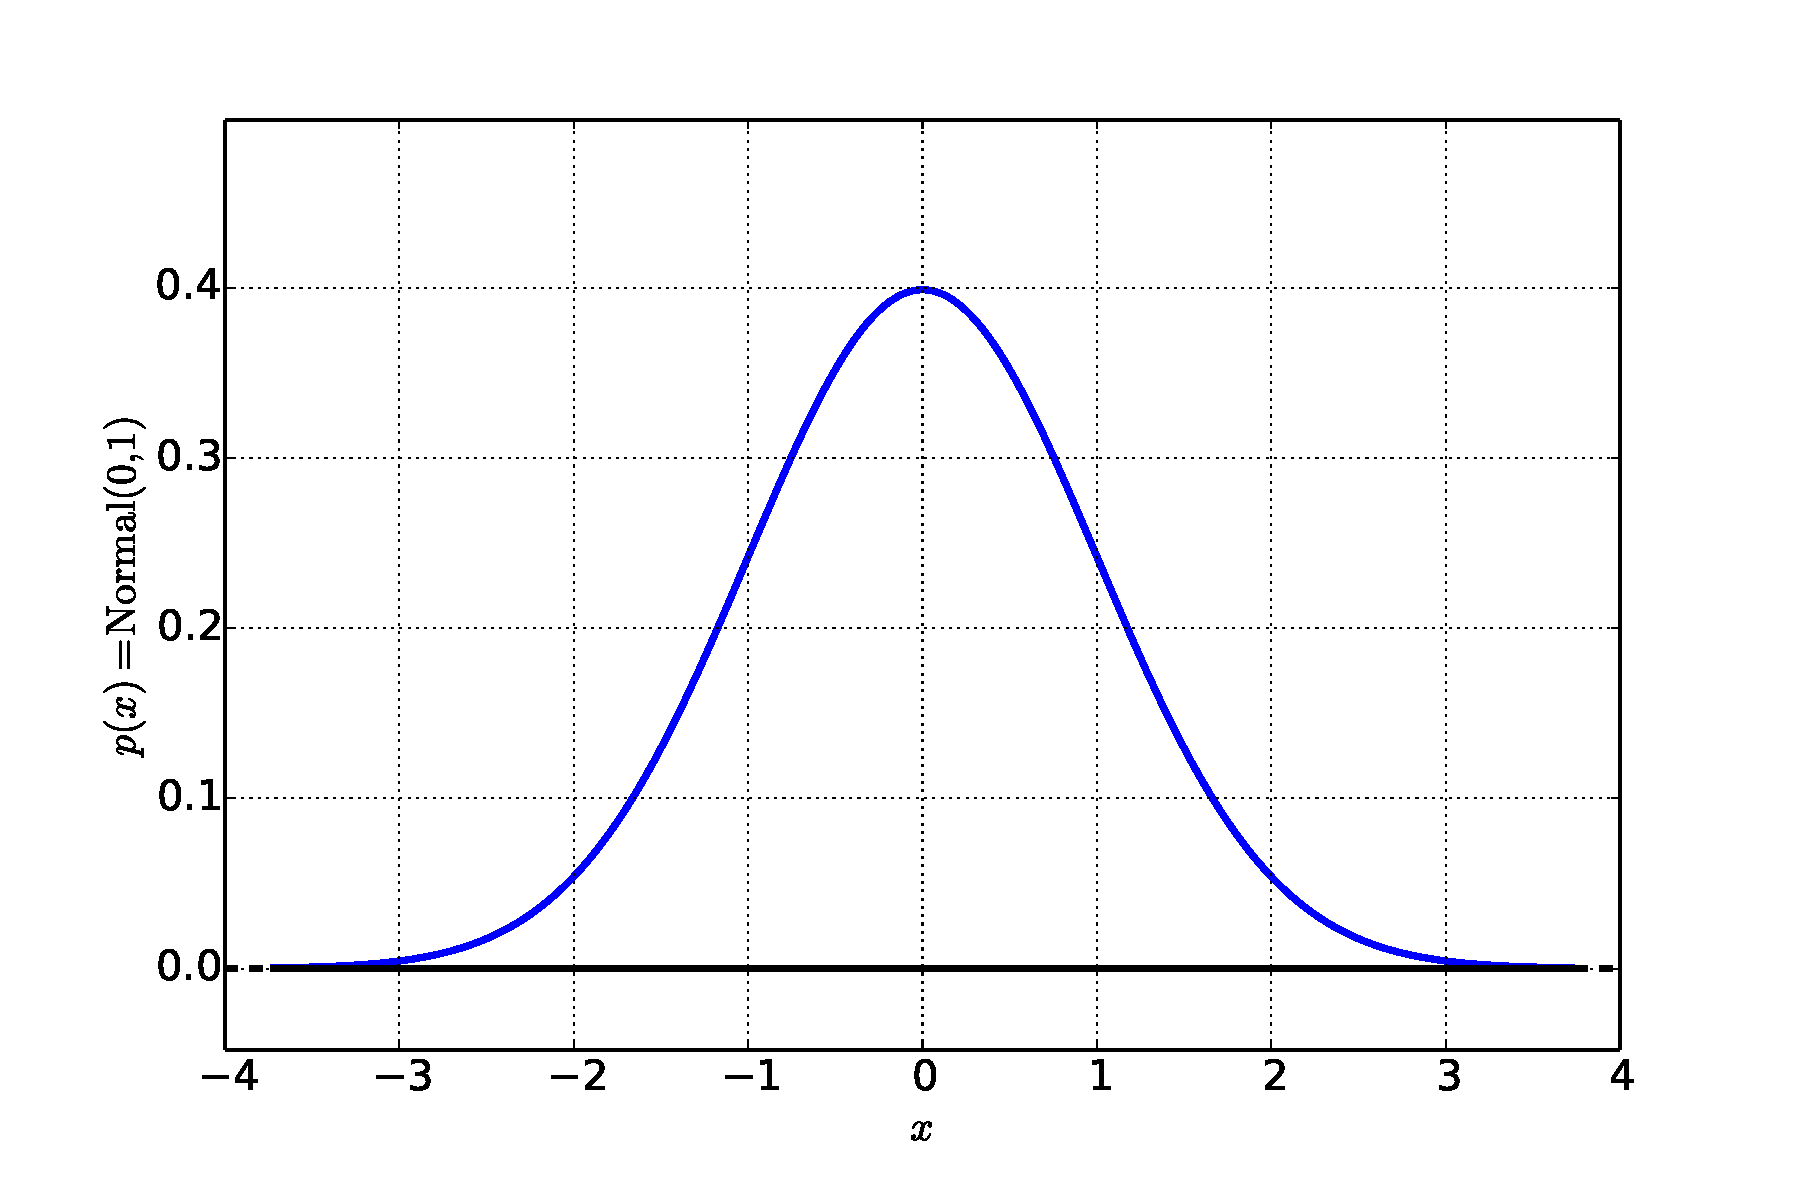
\includegraphics{gaussian1}
\caption{The Student's {\em t} distribution.}
\label{fig:tdist_appendix}
\end{figure}




\section{Poisson}

The Poisson distribution is a {\em discrete} distribution which gives the probability of rare events in time, given the average frequency, usually denoted with the greek letter $\lambda$.  If, for example, you observe an event 4 times a day on average (i.e. $\lambda=4$) such as receiving mail, or sneezing, or seeing buses on your street, then the probability on any given day of seeing this event $k$ times is given by this distribution:

\beqn
P(k) &=& \frac{\lambda^{k}e^{-\lambda}}{k!}
\eeqn

An example for different values of $\lambda$ is shown in Figure~\ref{fig:poisson}.

\begin{figure}
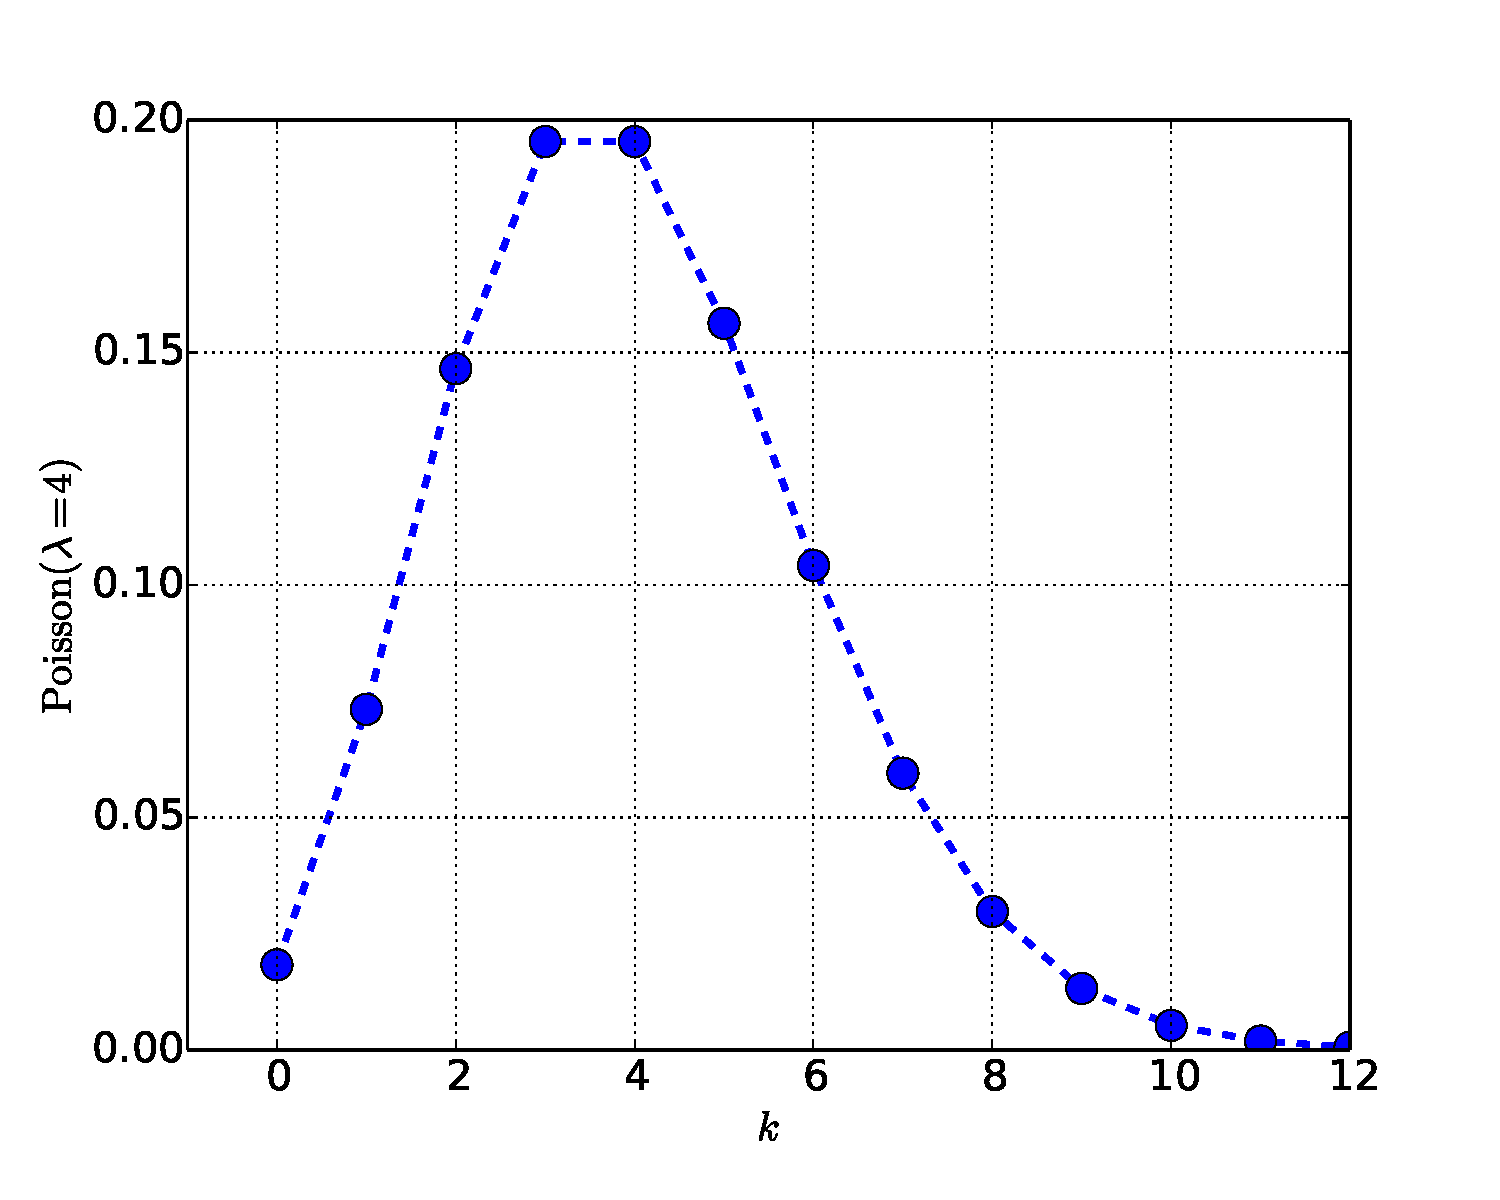
\includegraphics[width=4.8in]{distributions_poisson}
\label{fig:poisson}
\caption{Poisson distribution for several values of the parameter $\lambda$.}
\end{figure}

The Poisson distribution has the following properties:
\be
\i Mean : $\mu=\lambda$
\i Mode: largest integer less than or equal to $\lambda$ 
\i Standard deviation: $\sigma=\sqrt{\lambda}$
\ee

\subsubsection{The Poisson Distribution}

Here we're approximating a {\em discrete} distribution (poisson) with a \emph{continuous} one (normal).  The approximation is simply
\beqn
{\rm Poisson}(\lambda) = {\rm Normal}(\mu=\lambda,\sigma=\sqrt{\lambda})
\eeqn
Two examples which demonstrate the approximation are

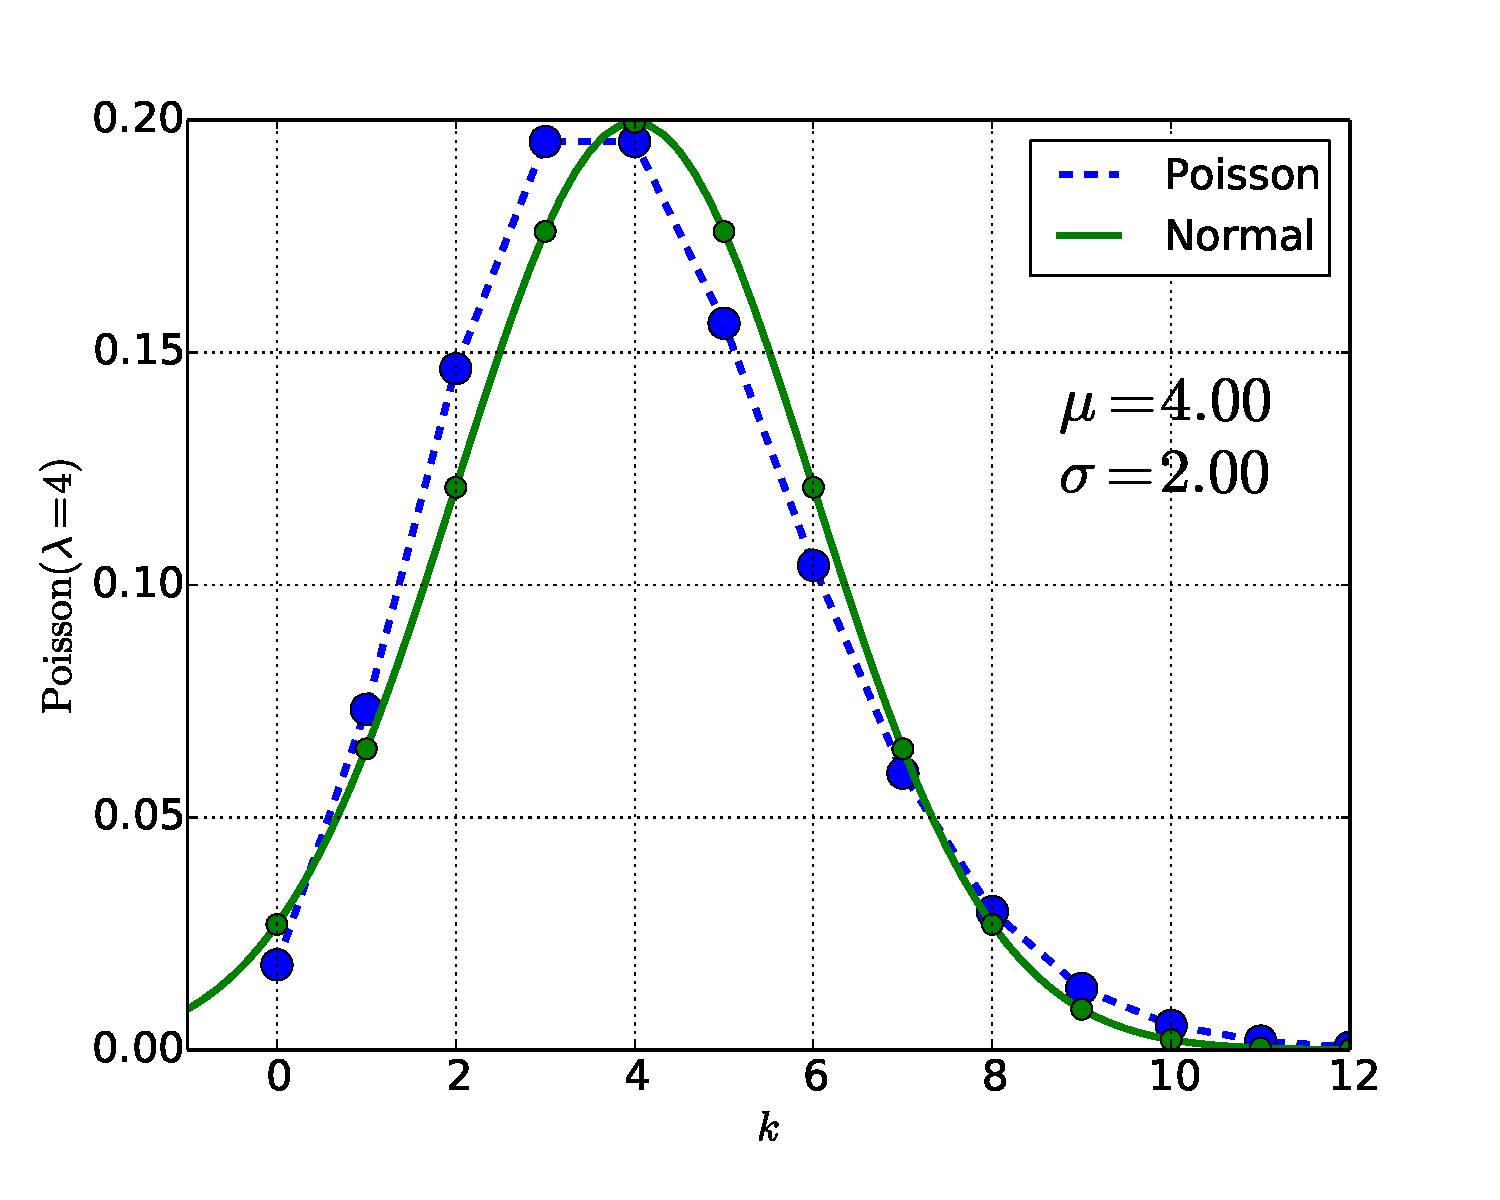
\includegraphics{poisson_normal1}

and

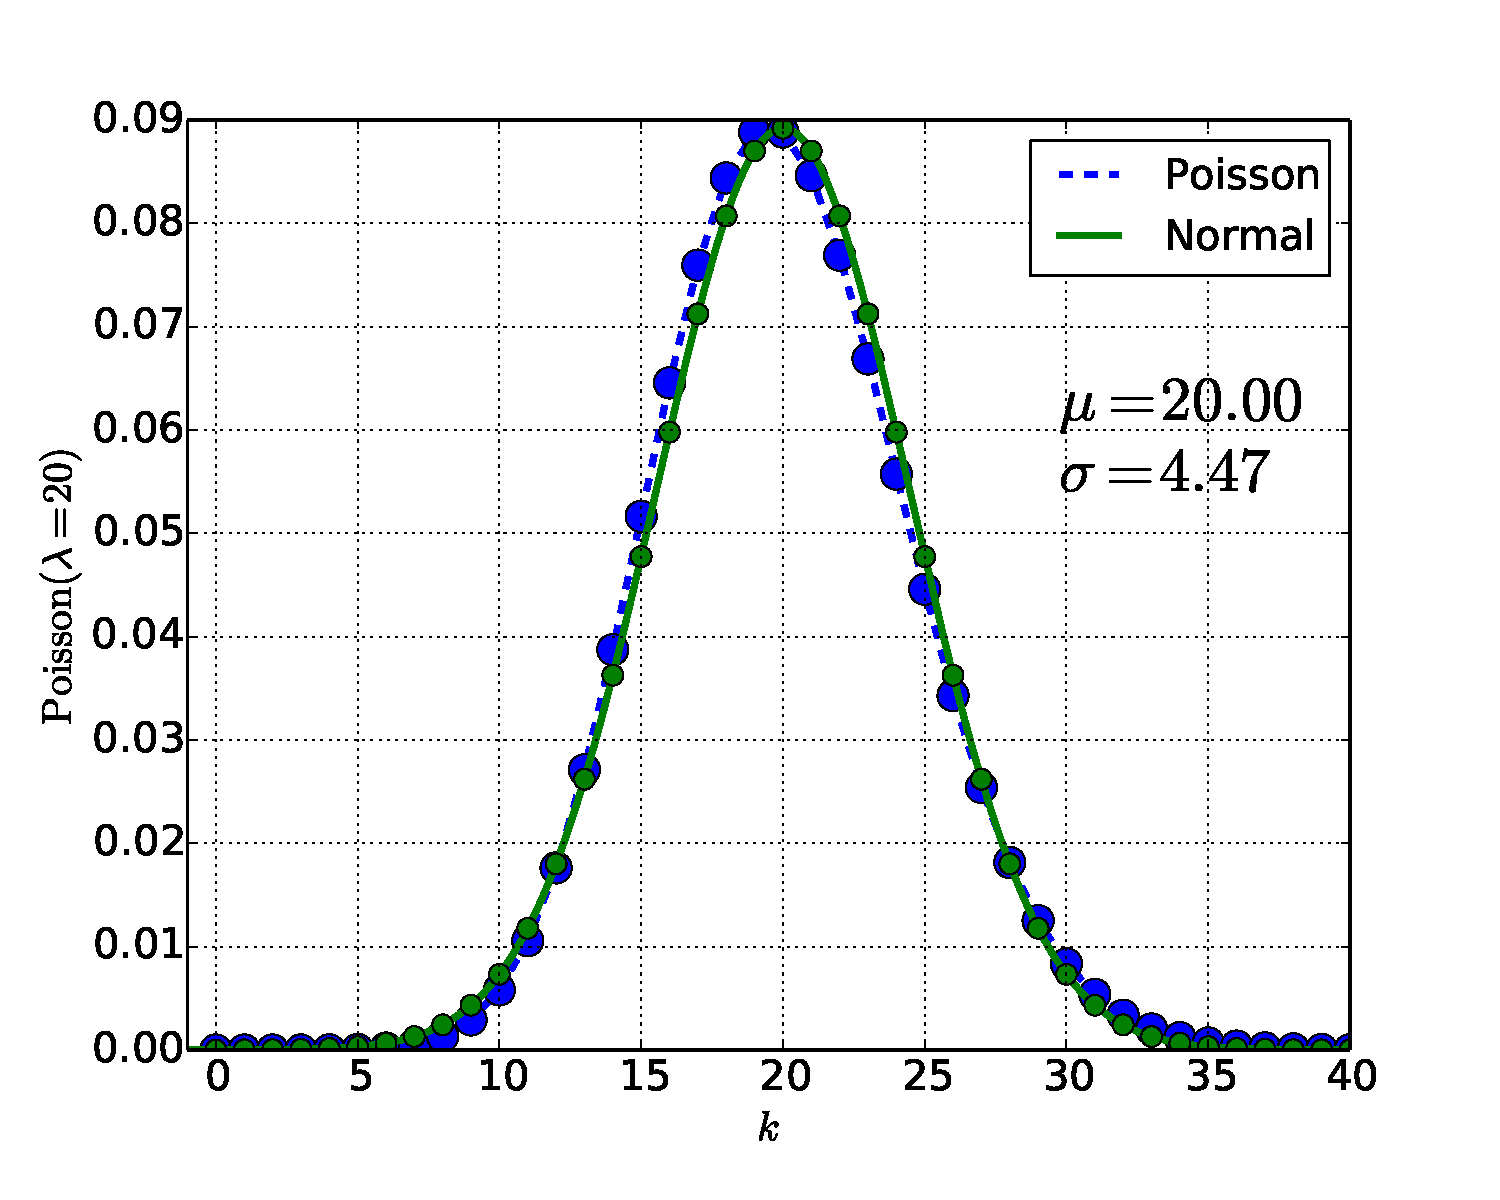
\includegraphics{poisson_normal2}

\section{Cauchy}

\section{F}

}
